\begin{table}[t]
    \rowcolors{2}{gray!25}{white}
    % \setlength\arrayrulewidth{0pt}
    \centering
    \resizebox{\textwidth}{!}{%
    \begin{tabular}{ c c c c c c }
        \toprule \textbf{Language Workbench} & \textbf{Modularization Supp.} & \textbf{Precompiled Feature Supp.} & \textbf{Native IDE gen.} & \textbf{LSP/DAP Gen.} & \textbf{LSP/DAP Mod.} \\
        \midrule
        JustAdd & \circleleft & \circlewhite & \circlewhite & \circlewhite & \circlewhite \\
        Melange & \circleblack & \circlewhite  & 3rd party (EMF) & $\filledstar$ & $\filledstar$ \\
        MontiCore & \circleleft & \circleleft & \circleblack & \circlewhite & \circlewhite \\
        MPS & \circleblack & \circlewhite   & \circleblack & $\filledstar$ & $\filledstar$ \\
        Rascal & \circlewhite & \circlewhite & \circleblack & \circlewhite & \circlewhite \\
        Spoofax & \circleblack & \circleleft  & \circleblack & $\filledstar$ & $\filledstar$ \\
        Xtext & \circlewhite & \circleleft  & \circleblack & \circleblack & \circlewhite \\
        Neverlang & \circleblack & \circleblack & \circlewhite & \FiveStarConvex & \FiveStarConvex \\
        \bottomrule
    \end{tabular}
    }
    \caption*{Comparison of language workbenches in terms of modularization, precompiled feature support, native IDE generation, LSP generation, and LSP modularization.}
    \label{tab:lw-comparison}
\end{table}

The primary aim of this project is to develop a Universal \textbf{Language Server Protocol}\footnote{https://microsoft.github.io/language-server-protocol} (LSP) and \textbf{Debugger Adapter Protocol}\footnote{https://microsoft.github.io/debug-adapter-protocol} (DAP) for modular language workbenches (LWs). This endeavor seeks to address significant gaps and challenges developing LSPs and DAPs in the current landscape of language workbenches, particularly in the areas of modularization, composition, and interoperability. Current language workbenches such as Melange~\cite{Degueule15}, MontiCore~\cite{Krahn10}, Spoofax~\cite{Visser10}, and MPS~\cite{Volter11, Voelter12} have made significant strides in supporting modularization, composition, and IDE integration.
The table above provides a comparison of various language workbenches in terms of their support for modularization, precompiled feature support, native IDE generation, LSP generation, and LSP modularization. The $\CIRCLE$ symbol indicates full support, $\Circle$ partial support, $\LEFTcircle$ limited support and \FiveStarConvex my contribution, which can be extended to all LWs that support at least component modularization (identified by $\filledstar$).
The second column indicates the level of support for modularization of artifacts and language features (more detail in~\hyperref[project-description]{Project Description} section). The third column indicates the level of support for precompiled features, the importance of this feature lies in the fact that an artifact can be used by several features being compiled once, and that one feature can be used among several projects without the recompilation step.  The fourth column indicates the level of support for native IDE generation, this is because many LWs are supported by the existence of some IDE and thus allow IDE generation for languages developed for IDE that host them.
The generation and modularizazion of LSP and DAP is trivial shown by the fifth and sixth columns, respectively.
However, their approaches are often fragmented and lack a standardized method for LSP and DAP generation and modularization, as shown in table.
Neverlang~\cite{Cazzola15c, Cazzola14c}, developed at the \texttt{ADAPT-Lab}\footnote{https://di.unimi.it/it/ricerca/risorse-e-luoghi-della-ricerca/laboratori-di-ricerca/adapt-lab} of the Università degli Studi di Milano, being a comprehensive framework for language composition and modularization that supports the development of language product lines~\cite{Cazzola15f, Cazzola21b} (LPLs), is a prime candidate for the implementation of the proposed LSP and DAP. The project will leverage the existing capabilities of Neverlang to develop a universal LSP and DAP that can be used across different programming languages and IDEs. This will enable developers to create external domain-specific languages~\cite{Fowler10} (DSLs) and general-purpose languages (GPLs) more effectively and efficiently, enhancing the overall development experience and productivity.


\hfill \break
The project aims to achieve the following objectives:

\hfill \break
\noindent
\textbf{Aim 1: Improve IDE and LSP Generation}
\hfill \break
\textit{Integrated Development Environment} generation and support for the \textit{Language Server Protocol} are essential for the practical use of domain-specific languages (DSLs). While some language workbenches like Xtext~\cite{Bettini13b} support LSP generation~\cite{Barros22}, many do not, limiting their usability across different editors and IDEs.
\hfill \break
\textbf{Relevance:} By establishing a universal protocol for LSP and DAP, this project aims to bridge the gap, enabling language workbenches to generate IDE support and LSPs more seamlessly. This will ensure that languages developed using these workbenches can be used in any IDE that supports these protocols, enhancing their accessibility and utility.

\hfill \break
\noindent
\textbf{Aim 2: Facilitate LSP and DAP Modularization}
\hfill \break
LSP and DAP modularization are not widely supported by current language workbenches~\cite{Bunder19a}. This feature is crucial for allowing different language components to communicate and function cohesively within an IDE.
\hfill \break
\textbf{Relevance:} Implementing support for LSP and DAP modularization will allow for better integration and interaction of various language features, thereby improving the overall development experience and capability of language workbenches. This aligns with the needs for more sophisticated and integrated language development tools as highlighted in the contemporary research and development literature.

\hfill \break
\noindent
\textbf{Aim 3: Reduce to $\mathcal{L} \times 1$ the number of combinations to support $\mathcal{L}$ languages}

\begin{figure}[t]
    \centering
    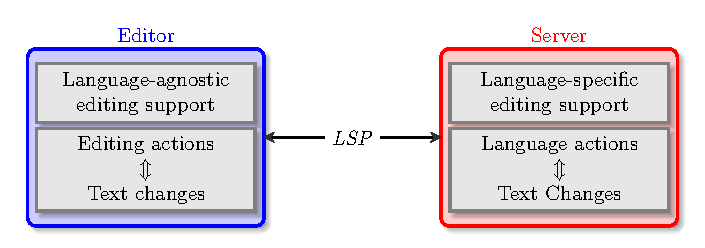
\includegraphics[width=0.75\linewidth]{figs/lsp_agnostic.pdf}
    \caption{LSP and DAP approach for programming languages.}
    \label{fig:agnostic}
\end{figure}

\hfill \break
Before the advent of LSP and DAP, developers had to implement language support for each editor separately, having the number of combinations to support $\mathcal{L}$ languages in $\mathcal{L} \times \mathcal{E}$, where $\mathcal{E}$ is the number of editors.
Currently, the number of combinations to support $\mathcal{L}$ languages is $\mathcal{L} + \mathcal{E}$~\cite{Rodriguez-Echeverria18a}, as the Microsoft LSP and DAP are editor-agnostic, as shown in Figure~\ref{fig:agnostic}. This project aims to reduce the number of combinations to $\mathcal{L} \times 1$, by developing a universal LSP and DAP that can be used across different programming languages and IDEs.
\hfill \break
\textbf{Relevance:} Reducing the number of combinations required to support multiple languages will simplify the development process and make it more efficient. This will enable developers to create language support more quickly and effectively, enhancing the overall productivity and usability of language workbenches.

\hfill \break
\noindent
\textbf{Aim 4: Leverage Neverlang for LSP and DAP in LPL Development}
\hfill \break
Neverlang's capabilities for language composition and modularization make it an ideal platform for developing a universal LSP and DAP that caters to a variety of language needs. By leveraging Neverlang's LPL development features~\cite{Cazzola20}, the project will establish a reusable core for LSP and DAP functionalities, allowing for the creation of product line variations tailored to specific programming language requirements. This will significantly reduce development time and effort for creating LSPs and DAPs for new languages within the product line.
\hfill \break
\textbf{Relevance:}  Developing a core reusable base for LSP and DAP functionalities through Neverlang's LPL features will streamline the creation of new language support. This fosters a more efficient and scalable approach to LSP and DAP development, aligning perfectly with the core principles of software product lines.

